
\newpage

\section{Generative Tasks \& Evaluation}

    \subsection{Task Generativi}

        I modelli linguistici possono essere utilizzati per affrontare diversi task generativi, tra cui la traduzione automatica, la classificazione e il question answering.

        \subsubsection{Machine Translation (MT)}   

            \begin{wrapfigure}{r}{0.6\textwidth}
                \vspace{-30pt}
                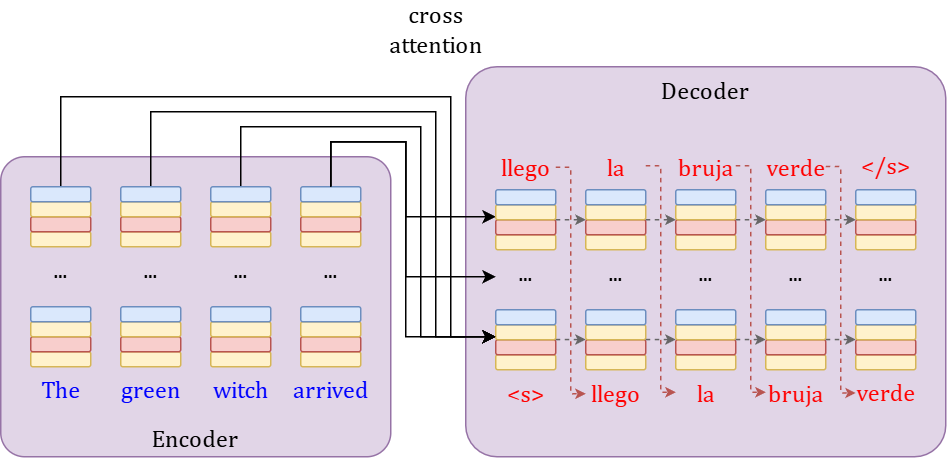
\includegraphics[width=1\linewidth]{imgs/schema_11_1.png}
                \label{fig:fig111}
            \end{wrapfigure}
        
            Il task di Machine Translation consiste nella traduzione automatica di testo operata da modelli \textit{encoder-decoder} o \textit{decoder-only}. Le lingue condividono caratteristiche universali, ma presentano differenze fondamentali che il modello deve gestire, come l'ordinamento delle parole (SVO, SOV, ecc.), divergenze lessicali (sinonimi), tipologie morfologiche e densità referenziale (ad esempio, l'omissione dei pronomi in italiano rispetto all'inglese).

            \paragraph{Strategie di Decoding} Nella fase di generazione del testo, l'obiettivo è trovare la sequenza di token più probabile. La \textit{greedy search} sceglie il token più probabile ad ogni passo, offrendo una soluzione localmente ottimale ma non necessariamente globale. Poiché la ricerca esaustiva è impraticabile a causa dell'enorme spazio delle soluzioni, si adottano strategie avanzate:

            \begin{itemize}
                \item \textbf{Beam Search}: Ad ogni step, per ciascuna delle $k$ ipotesi, si calcola la probabilità dei token successivi e si mantengono solo le $k$ sequenze con probabilità cumulativa maggiore.
                Lo \textit{score} di una sequenza generata è dato dalla somma delle log-probabilità; poiché la natura additiva dello score penalizzerebbe le sequenze più lunghe, si applica un fattore di normalizzazione basato sulla lunghezza $T$ della sequenza:
                $$score(y) = \frac{1}{T} \sum_{i=1}^{T} -\log P(y_i|y_1,...,y_{i-1}, x)$$

                \item \textbf{Minimum Bayes Risk (MBR) Decoding}: Strategia che utilizza esplicitamente una metrica di valutazione ($util$) per misurare la bontà di una traduzione. Piuttosto che scegliere la traduzione più probabile, l'MBR seleziona quella con l'errore atteso più basso rispetto ad un set $Y$ di traduzioni candidate:
                $$\hat{y} = argmax_{y \in Y} \sum_{c \in Y} util(y,c)$$
            \end{itemize}

        \subsubsection{Text Classification e Question Answering}
        
            Task tradizionalmente discriminativi, come la \textit{Text Classification} (es. sentiment analysis, fake news detection), possono essere risolti in ottica generativa tramite \textit{prompting} o \textit{constraint decoding} (forzando il modello a generare solo le etichette valide).

            Il \textbf{Question Answering (QA)} prevede due approcci principali:
            
            \begin{itemize}
                \item \textit{Extractive}: Individuare la sottosequenza esatta che contiene la risposta all'interno di un contesto fornito.
                \item \textit{Abstractive}: Generare testualmente una risposta a partire da un contesto (Open QA).
            \end{itemize}
            
            Spesso i sistemi QA si focalizzano su \textit{factoid questions} (domande su fatti specifici). Tuttavia, demandare il task di QA a un LLM in forma puramente generativa comporta un alto rischio di \textit{allucinazioni} (risposte non fattuali). Per mitigare questo rischio, la conoscenza parametrica del modello viene spesso affiancata a sistemi di Information Retrieval (architetture RAG).

    \newpage

    \subsection{Valutazione dei Modelli Generativi}

        La valutazione stima la bontà del testo generato, idealmente confrontandolo con un corpus di frasi \textit{golden} o \textit{reference}. Le due proprietà principali valutate sono l'\textit{Adequacy/Faithfulness} (fedeltà al significato) e la \textit{Fluency} (correttezza grammaticale).

        Le tipologie di valutazione si dividono in: Umana, Automatica e LLM as a judge. La valutazione umana, seppur costosa, è utile quando manca una \textit{golden answer} e permette di ottenere \textit{score} numerici o \textit{ranking} di alta qualità.

        \subsubsection{Metriche di Valutazione Automatica}
    
            Confrontano la risposta generata (\textit{hypothesis}, $h$) con una o più frasi di \textit{reference} ($r$). Possono basarsi sulla sovrapposizione dei caratteri/parole o sulla similarità degli \textit{embedding}:

            \begin{itemize}
                \item \textbf{chrF (Character F-score)}: Misura la sovrapposizione di $k$-grams di caratteri. Calcola la media delle \textit{precision} (chrP) e delle \textit{recall} (chrR) calcolando una F1-score pesata dal parametro $\beta$:
                $$chrF\beta = (1+\beta^2)\frac{chrP \cdot chrR}{\beta^2 \cdot chrP + chrR}$$
                
                \item \textbf{BLEU (BiLingual Evaluation Understudy)}: Metrica orientata alla \textit{precision} basata sulla sovrapposizione di parole (n-grams). È moltiplicata per una \textit{Brevity Penalty} (BP) per penalizzare frasi troppo corte:
                $$BLEU(H,R) = BP \cdot exp\left(\frac{1}{N}\sum_{n=1}^{N} \log p_n(H,R)\right)$$
                
                \item \textbf{ROUGE}: Metriche orientate alla \textit{recall}. \textit{ROUGE-N} calcola precision e recall degli N-grammi comuni. \textit{ROUGE-L} ricerca la Longest Common Subsequence (LCS) tra hypothesis e reference.
                
                \item \textbf{METEOR}: Supera i limiti della sovrapposizione esatta considerando sinonimia, \textit{stemming} e l'ordine delle parole. Utilizza una formula basata su F-mean e una penalità.
                $$Score = F_{mean} * (1 - Penalty)$$
                
                \item \textbf{BERTScore}: Sposta la comparazione nello spazio degli embedding contestuali, calcolando la Pairwise Cosine Similarity tra i token generati e quelli di reference. La \textit{recall} del BERTScore è:
                $$R_{BERT} = \frac{1}{|x|} \sum_{x_i \in x} \max_{\tilde{x}_j \in \tilde{x}} x_i \cdot \tilde{x}_j$$
            \end{itemize}

        \subsubsection{LLM as a Judge}
        
            Tecnica in cui un LLM esperto (es. GPT-4, Claude) viene interrogato per valutare l'output generato da un altro modello. Formalmente, la valutazione $\mathcal{E}$ è espressa come:
            $\mathcal{E} \leftarrow P_{LLM}(x \oplus \mathcal{C})$
            dove $x$ è l'input da valutare, $\mathcal{C}$ è il contesto/template (che può richiedere una classificazione binaria, un confronto o una scala Likert), e $\oplus$ è l'operatore di concatenazione.

        \newpage

        \subsubsection{RAGAS}
        
            RAGAS è un framework basato su "LLM as a judge" specifico per valutare sistemi RAG (Retrieval-Augmented Generation). Valuta quattro metriche principali:
        
            \begin{figure}[H]
                \centering
                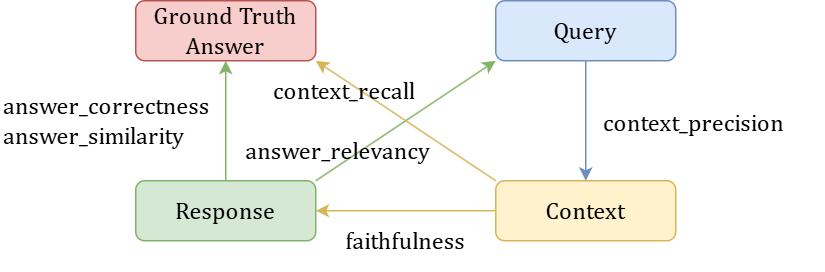
\includegraphics[width=0.8\linewidth]{imgs/schema_11_2.png}
                \label{fig:fig112}
            \end{figure}

            \begin{enumerate}
                \item \textbf{Context Recall}: Misura la proporzione di informazioni rilevanti (Ground Truth) recuperate con successo. 
                $$Context\_Recall = \frac{|GT \text{ claims attributed to the context}|}{|GT \text{ claims}|}$$

                \item \textbf{Context Precision}: Proporzione di \textit{chunk} rilevanti nel contesto recuperato, calcolata come media della $Precision@k$ per i risultati top $K$.
                
                \item \textbf{Faithfulness}: Accuratezza fattuale; verifica se le affermazioni della risposta sono supportate dal contesto fornito.
                $$Faithfulness = \frac{\# \text{ valid statements}}{\# \text{ statements}}$$
                
                \item \textbf{Answer Relevancy}: Misura la pertinenza della risposta calcolando la \textit{cosine similarity} tra la domanda originale ($E_o$) e un set di $N$ domande generate a partire dalla risposta ($E_{g_i}$).
                $$Answer\_Relevancy = \frac{1}{N} \sum_{i=1}^{N} \frac{E_{g_i} \cdot E_o}{||E_{g_i}|| ||E_o||}$$
            \end{enumerate}